%************************************************
\chapter{Grounded Learning of Knowledge Utility}
\label{chapter:grounded_learning_of_knowledge_utility}
%************************************************

Hypothetical type knowledge transframes are used by the deliberative
and reflective planning machines in order to infer the effects of
executing plans.  There is a distinction here made between the
\emph{factual} knowledge that is directly an abstraction of knowledge
grounded in the physical or deliberative planning machine knowledge
bases, which are not based on any learned action hypotheses, and the
\emph{counterfactual} knowledge that is inferred and supported by
hypotheses of the effects of resource executions that the AI has
either ``been told'' or has learned in the course of actually
executing those resources in different contexts.  In order to maintain
this distinction in the AI, different knowledge bases are used to
separate the factual knowledge from counterfactual knowledge.  Factual
knowledge is induced into factual type knowledge abstractions.  The
factually grounded knowledge bases include the visual, physical,
physical type, deliberative planning machine, and deliberative
planning machine type knowledge bases.  However, the addition of
factually grounded knowledge causes a loss of hypotheses from the
resource execution type knowledge transframe hypothesis spaces in both
the deliberative and reflective layers.  Each counterfactual event in
the counterfactual knowledge bases has a list of dependencies that
must maintain their support in order for the counterfactual knowledge
to continue to exist.  Dependencies in the AI have three types of
support that can be rearranged in order to maintain the support of
counterfactual knowledge events:
\begin{enumerate}
\item Resource execution transframe preconditions.
\item Resource execution.
\item Resource execution transframe change hypotheses.
\end{enumerate}
If any of these three types of supports loses its hypothetical factual
grounding, this loss of hypothetical factual grounding causes the
dependency to become \emph{invalidated}.  Once a dependency has become
invalidated, it has a chance to find new hypothetical grounding before
it becomes \emph{unsupported}.  Counterfactual event knowledge is
notified when a dependency has become unsupported, causing the
counterfactual events to be removed from the counterfactual event
knowledge bases.  Also, as some counterfactual knowledge may form
hypothetical grounding of further dependencies of further
counterfactual event knowledge, the loss of support for a dependency
can cause a chain reaction through events and their dependent
dependencies.  In this way, additional factual knowledge refines and
reduces the hypothetical support of transframe changes, invalidating
hypothetical dependencies, and potentially causing the loss of support
for counterfactual knowledge that has been inferred in the
counterfactual event knowledge bases of the deliberative and
reflective layers of the AI.

\section{Learning from Being Told Deliberative Plans}

In {\mbox{\autoref{table:a_plan_learned_from_being_told}}} on page
{\mbox{\pageref{table:a_plan_learned_from_being_told}}}, there is an
assertion at the end of the plan for reactive resource execution that
the AI has been told: ``Assert a cube is sitting on a pyramid.''  When
the AI initially learns a plan from being told, it does not yet have
any factual knowledge to eliminate any hypotheses about the effects of
the resource executions.  When the AI learns plan knowledge from being
told, the asserted type knowledge in the plan are added to the
resource execution hypothesis spaces before the assertion.  In this
case, the resource execution immediately before the assertion is:
``Drop and wait for block to fall.''  Therefore, the AI does not
eliminate any hypotheses from the resource execution hypothesis spaces
but instead augments the potential \emph{change features} of this
resource's hypothesis spaces with this new \emph{add} change.  In
other words, the hypothesis space for the resource execution is
augmented to include all consistent hypotheses that both predict this
change and that do not predict this change.  Since the AI has no
previous factual knowledge about this change, it is capable of
predicting both possibilities, each with different sets of supporting
hypotheses: (1) that this feature is added when the resource is
executed in the given preconditions or (2) that this feature is not
added in the given preconditions.
{\mbox{\autoref{figure:inference_of_physical_knowledge}}} shows how
the augmented hypothesis space of this resource execution causes the
imaginative inference that will result in the future counterfactual
knowledge: ``A cube is sitting on a pyramid.''  Also, notice how the
three different types of dependencies relate the factual physical type
knowledge to this counterfactual physical type knowledge through the
potential reactive resource execution in order to predict the
hypothetically supported stack of blocks in the future.
\begin{figure}[h]
\centering
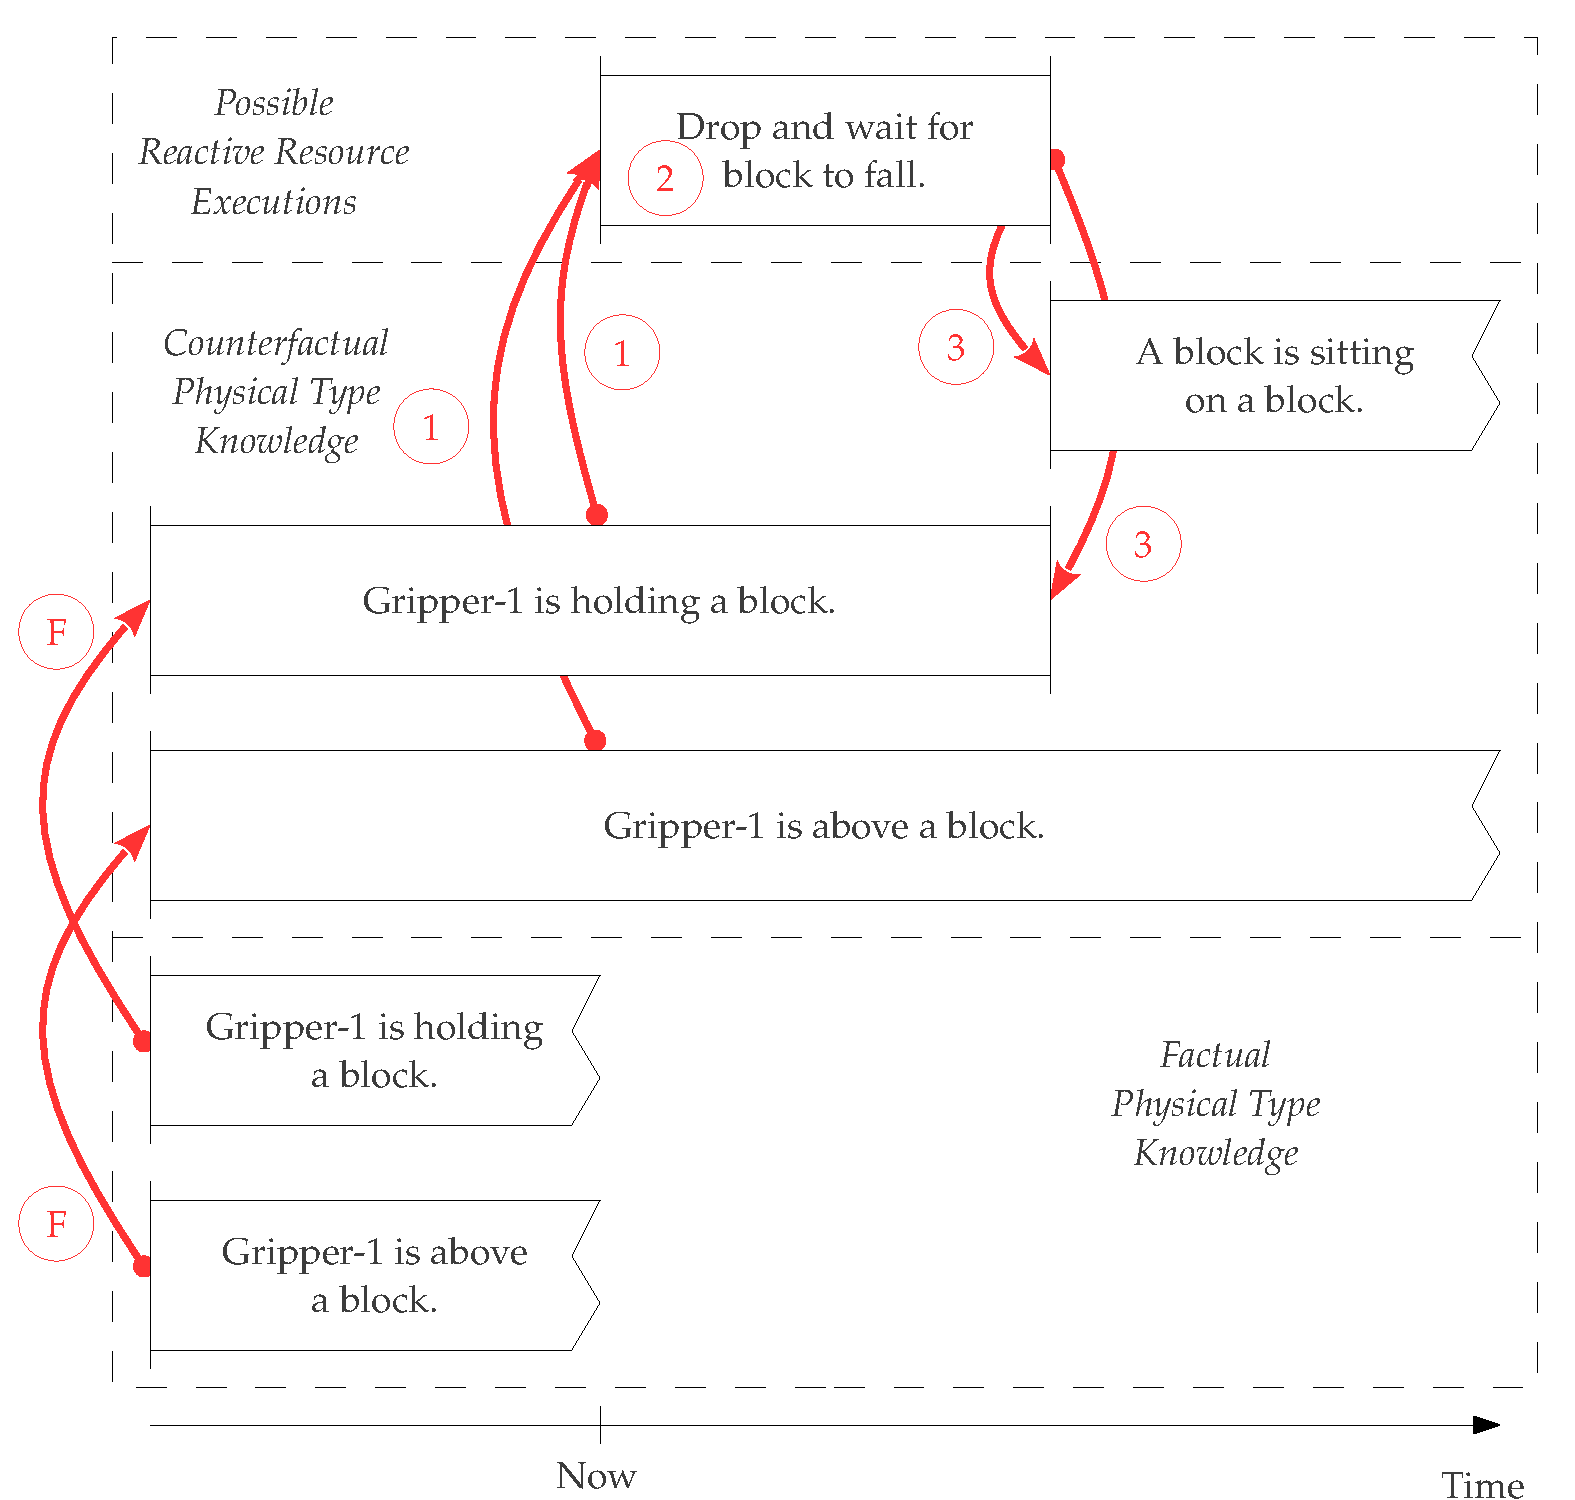
\includegraphics[width=12cm]{gfx/inference_of_physical_knowledge}
\caption[Inference of counterfactual physical type knowledge from
  factual physical type knowledge.]{Inference of counterfactual
  physical type knowledge from factual physical type knowledge.
  Rectangular boxes represent events over time.  Some events have a
  jagged right edge to indicate that this event has no ending time.
  Curved arrows represent different dependency relationships: (F)
  factual, (1) precondition, (2) potential resource execution, and (3)
  hypothetical change.  Preconditions, potential resource activations,
  and hypothetical changes form the three possibly unsupported parts
  of a dependency.  Factual dependencies cannot lose support because
  they are derived directly from factual events.}
\label{figure:inference_of_physical_knowledge}
\end{figure}
{\mbox{\autoref{figure:inference_of_deliberative_planning_machine_knowledge}}}
shows how the three different types of dependencies analogously relate
factual deliberative planning machine type knowledge to counterfactual
deliberative planning machine type knowledge through potential
deliberative planning resource executions in order to predict
hypothetical plan failure in the future.
\begin{figure}[h]
\centering
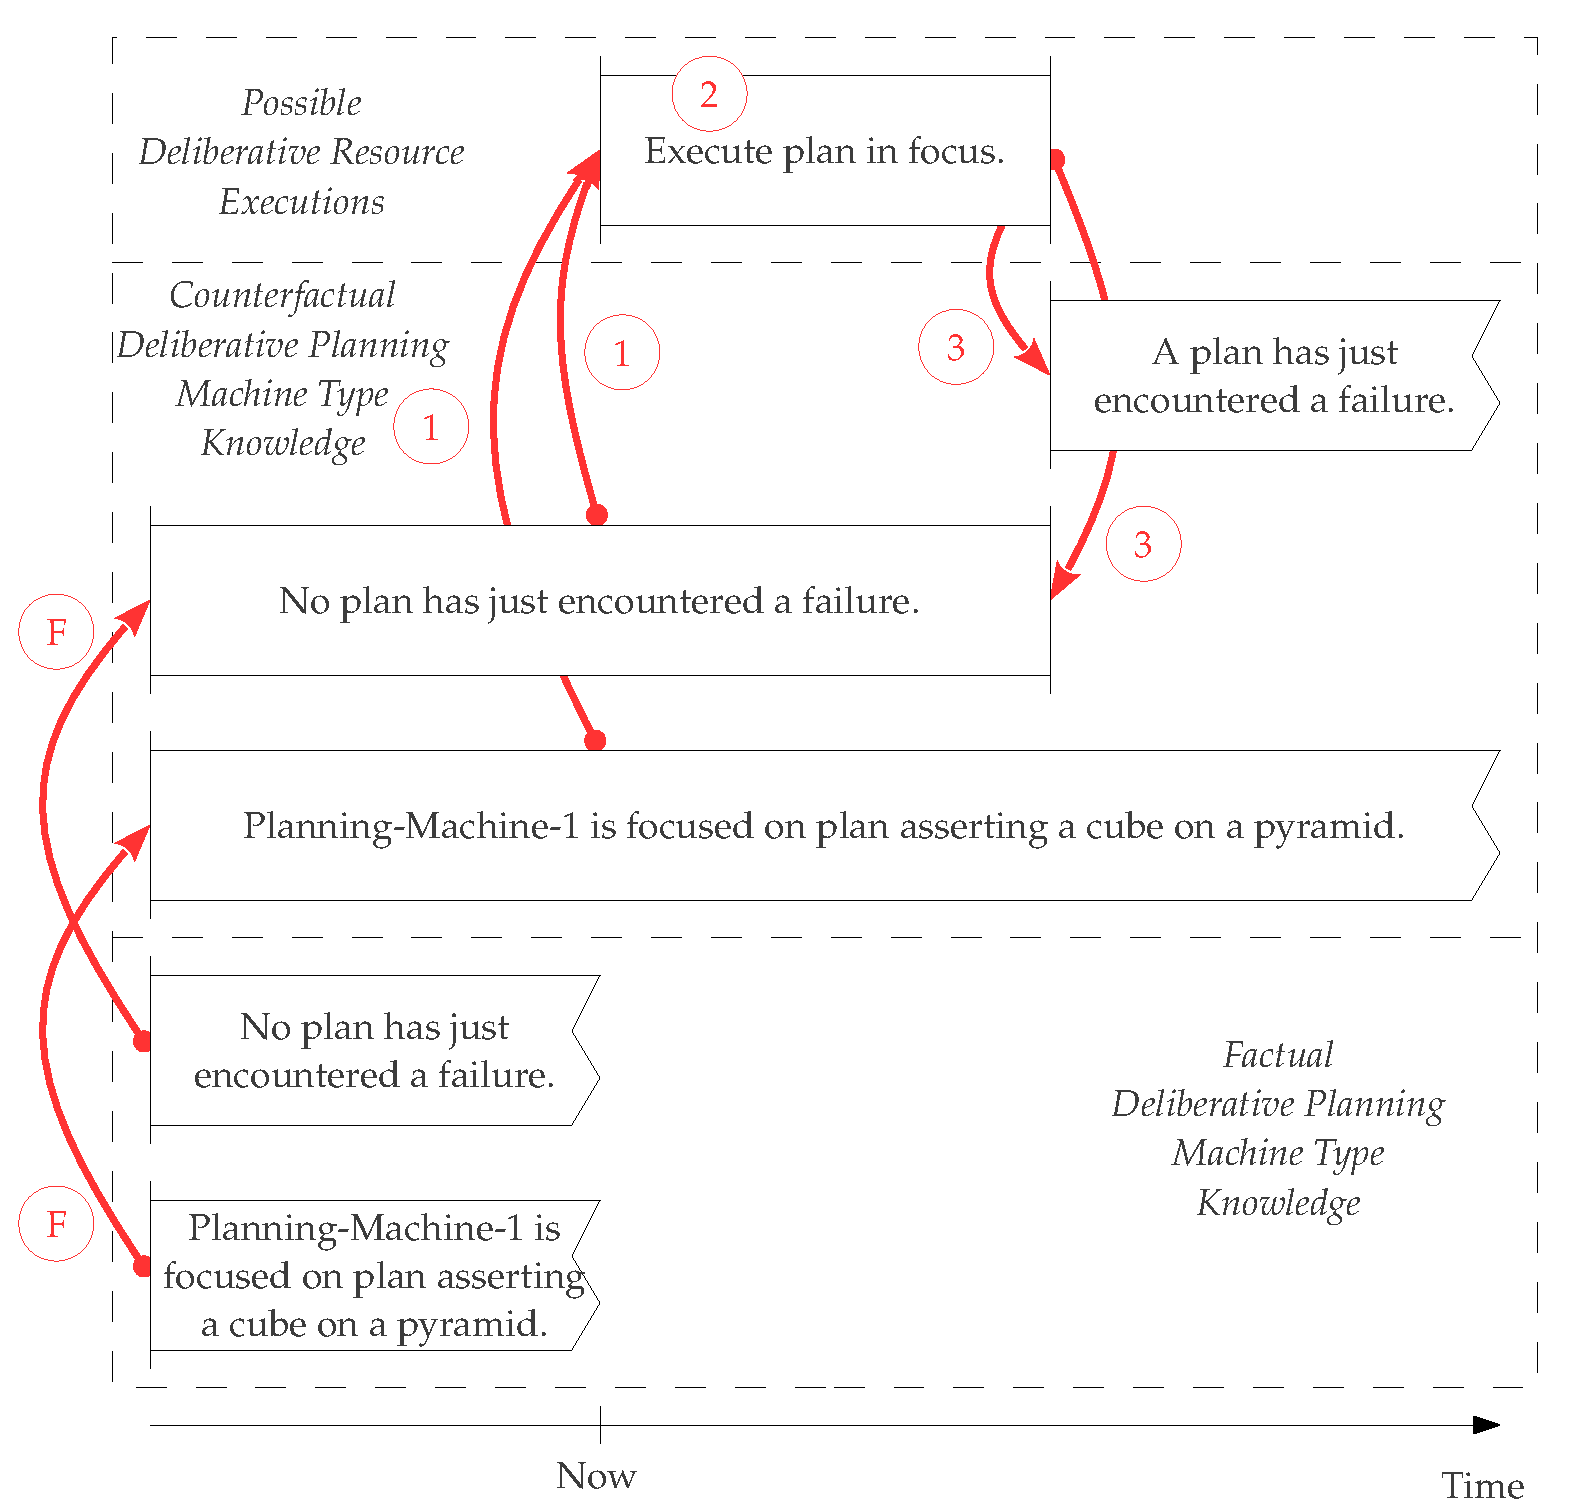
\includegraphics[width=12cm]{gfx/inference_of_deliberative_planning_machine_knowledge}
\caption[Inference of counterfactual deliberative planning machine
  type knowledge from factual deliberative planning machine type
  knowledge.]{Inference of counterfactual deliberative planning
  machine type knowledge from factual deliberative planning machine
  type knowledge.  Rectangular boxes represent events over time.  Some
  events have a jagged right edge to indicate that this event has no
  ending time.  Curved arrows represent different dependency
  relationships: (F) factual, (1) precondition, (2) potential resource
  execution, and (3) hypothetical change.  Preconditions, potential
  resource activations, and hypothetical changes form the three
  possibly unsupported parts of a dependency.  Factual dependencies
  cannot lose support because they are derived directly from factual
  events.}
\label{figure:inference_of_deliberative_planning_machine_knowledge}
\end{figure}


\section{Propagating Loss of Hypotheses to Counterfactual Inferences}

Plan knowledge that the AI has been told can inform its hypothesis
spaces for the potential changes that resource executions will cause,
allowing the AI to imagine both successful and unsuccessful
accomplishment of the goal condition of ``A block is sitting on a
block'' with different hypothetical supports.  When the AI executes
the resource, it refines these hypothesis spaces that predicts these
changes given the factual preconditions and effects of the actual
resource execution.  The refinement of hypothesis spaces has the
potential to eliminate the hypotheses that have supported previous
counterfactual inferences.  In order to correct counterfactual
inferences when hypotheses are removed from hypothesis spaces, every
individual hypothesis in each resource execution transframe change
hypothesis space has a list of \emph{removal callbacks} that are
called if the hypothesis is ever removed from the hypothesis space.
So, when the hypothesis space is refined in light of new factual
evidence, dependencies that are supported by these hypotheses are
notified that they have become \emph{invalidated}.  When a dependency
has become invalidated, it has a chance to reconfigure its
hypothetical support, so that it can still predict the same
hypothetical change, and thus, still support the counterfactual
knowledge that depends upon it.  Here are the basic steps of the
grounded hypothesis refinement process that corrects and removes
unsupported counterfactual knowledge in light of new evidence and
refined hypothesis spaces:
\begin{enumerate}
\item When a resource execution transframe change hypothesis space is
  refined, removing hypotheses, registered callbacks for each of these
  hypotheses are called, invalidating the dependencies that are
  supported by these hypotheses.
\item Invalidated dependencies check to see if the resource execution
  transframe change hypothesis space still contains hypotheses that
  will support the change given the preconditions for the possible
  resource execution.
\item If the invalidated dependency can find new hypothetical support
  for the resource execution transframe change, it marks itself as
  valid and no counterfactual events are modified as the dependency
  has found new supporting hypotheses.
\item If the invalidated dependency cannot find new hypothetical
  support for the resource execution transframe change, it becomes
  unsupported and marks dependent counterfactual knowledge to be
  unsupported and removed from the counterfactual knowledge base.
\item If a counterfactual event loses the support of a dependency and
  is removed from the counterfactual knowledge base, those
  dependencies that are supported by these counterfactual events as
  preconditions are invalidated, causing the propagation of the
  refined hypothesis spaces to correct further counterfactual event knowledge.
\end{enumerate}

In this way, as hypothesis spaces are refined and hypotheses are
eliminated due to new factual evidence, the effects on the
counterfactual knowledge is minimized by first invalidating the
dependencies, allowing them to rearrange their supports where
possible, before dependencies give up and declare themselves as
unsupported to their dependent counterfactual events.

\section{Losing and Searching for New Hypothetical Support}

When the AI first imagines that executing its plan will result in ``A
cube is sitting on a pyramid,'' this counterfactual event is
associated with the newly created dependency shown in
{\mbox{\autoref{table:physical_dependency}}}.
\begin{table}[h]
\centering
\begin{tabular}{c}
  A Supported Dependency for Counterfactual \\
  Physical Type Knowledge Event \\
  ``A cube is sitting on a pyramid.'' \\
  \begin{tabular}{|p{3cm}|p{6cm}|}
    \hline
    \emph{possible resource execution:} & Drop and wait for block to fall. \\
    \hline
    \emph{preconditions:}               & \\
    \hline
    \emph{add hypotheses:}              & \emph{True} \\
    \hline
  \end{tabular}
\end{tabular}
\caption[A dependency for a counterfactual physical type knowledge
  event given no factual evidence.]{A dependency for a counterfactual
  physical type knowledge event given no factual evidence.  Notice
  that since this knowledge has ``been told'' to the AI without any
  experience executing this action, the hypothesis space has not been
  refined and the most general hypothesis, which predicts \emph{True}
  in all preconditions, is the only supporting hypothesis for this
  counterfactual event.}
\label{table:physical_dependency}
\end{table}
When the AI actually executes the ``Drop and wait for block to fall
resource'', the hypothesis space for the addition of ``A cube is
sitting on a pyramid'' is refined by removing those hypotheses that
are no longer consistent with the factual event knowledge.  The
hypothesis space reflects that in the specific preconditions of the
execution, the change did not occur.  However, the AI is not sure
about other possible preconditions.  In this case, the most general
hypothesis, which is \emph{True} in all preconditions, has been
removed from the hypothesis space.  This causes the dependency shown
in {\mbox{\autoref{table:physical_dependency}}} to become invalidated.
The dependency then attempts to find new hypothetical support for its
predicted change.  In this case, the dependency is not able to
reconfigure its support in order to mark itself as once again valid,
so the dependency becomes unsupported and removes the unsupported
counterfactual event that depends upon it.  The unsupported dependency
due to the loss of the most general hypothetical support is shown in
{\mbox{\autoref{table:physical_reconfigured_dependency}}}.
\begin{table}[h]
\centering
\begin{tabular}{c}
  An Unsupported Dependency for Counterfactual \\
  Physical Type Knowledge Event \\
  ``A cube is sitting on a pyramid.'' \\
  \begin{tabular}{|p{3cm}|p{6cm}|}
    \hline
    \emph{possible resource execution:} & Drop and wait for block to fall. \\
    \hline
    \emph{preconditions:}               & $A$: Gripper-1 is holding a block. \\
                                        & $B$: Gripper-1 is above a cube. \\
    \hline
    \emph{add hypotheses:}              & ${\neg}A \wedge B$ \\
                                        & $A \wedge {\neg}B$ \\
                                        & ${\neg}A \wedge {\neg}B$ \\
    \hline
  \end{tabular}
\end{tabular}
\caption[An unsupported dependency for a counterfactual physical type
  knowledge event after losing its original hypothetical support and
  attempting to reconfigure new support.]{An unsupported dependency
  for a counterfactual event after losing its original hypothetical
  support due to experience executing the reactive resource.  Note
  that this dependency has found a number of hypotheses that would
  provide support under different preconditions.}
\label{table:physical_reconfigured_dependency}
\end{table}

Initially the reflective layer of the AI has not been told any plans
that assert conditions of the deliberative planning machine type
knowledge.  This means that when the reflective layer imagines
executing the plan in focus, it does not predict a failure will occur.
However, when the AI has executed the plan to stack the cube on the
pyramid, this actually does result in a factual failure.  The AI
reflectively responds to the failure by imagining executing a new plan
for deliberative action.  The reflective layer infers the
counterfactual deliberative planning machine type knowledge shown in
{\mbox{\autoref{figure:inference_of_deliberative_planning_machine_knowledge}}}.
During this imaginative inference process, the reflective layer
creates the counterfactual event, ``A plan has just encountered a
failure'', which has the newly created dependency shown in
{\mbox{\autoref{table:deliberative_dependency}}}.
\begin{table}[h]
\centering
\begin{tabular}{c}
  A Supported Dependency for Counterfactual \\
  Deliberative Planning Machine Type Knowledge Event \\
  ``A plan has just encountered a failure.'' \\
  \begin{tabular}{|p{3cm}|p{6cm}|}
    \hline
    \emph{possible resource execution:} & Execute plan in focus. \\
    \hline
    \emph{preconditions:}               & $A$: No plan has just encountered a failure. \\
                                        & $B$: Planning-Machine-1 is focused on plan asserting a cube on a pyramid. \\
    \hline
    \emph{add hypotheses:}              & $A \wedge B$ \\
    \hline
  \end{tabular}
\end{tabular}
\caption[A dependency for a counterfactual deliberative planning
  machine type knowledge event given no factual evidence.]{A
  dependency for a counterfactual deliberative planning machine type
  knowledge event given the factual evidence of previously executing
  this deliberative resource once in the given deliberative planning
  machine type knowledge preconditions.}
\label{table:deliberative_dependency}
\end{table}
With the AI's new experience, it imagines executing another plan,
which asserts ``A pyramid is sitting on a cube.''  The execution of
the first plan is avoided due to the prediction of failure in the
reflective imaginative inference of counterfactual failure for this
plan.  When the new plan is selected, it finally succeeds in
accomplishing the physical goal condition: ``A block is sitting on a
block,'' demonstrating the abstract reflective imagination of plan
execution, in this case, helps to accomplish the primary physical goal
at hand.

